\section{Introduction}
\label{sec:intro}

Neural networks achieve high predictive accuracy in many tasks, but they are known to have two substantial weaknesses: First, neural networks are not robust against adversarial perturbations, i.e., semantically meaningless input changes that lead to wrong predictions \citep{szegedy2014, goodfellow2014}. 
Second, standard neural networks are unable to identify samples that are different from the ones they were trained on and tend to make over-confident predictions at test time \citep{ensemble_simple}. These weaknesses make them impracticable in sensitive domains like financial, autonomous driving or medical areas which require trust in predictions.



To increase trust in neural networks, models that provide predictions along with the corresponding uncertainty have been proposed. 
An important, quickly growing family of models is the Dirichlet-based uncertainty (DBU) family \citep{malini2018, malinin2019, sensoy2018, malinin2019ensemble, charpentier2020, graph_uncertainty, max_gap_id_ood, multifaceted_uncertainty, uncertainty-generative-classifier}. 
Contrary to other approaches such as Bayesian Neural Networks \citep{blundell2015, osawa2019, wesley2019}, drop out \citep{drop_out} or ensembles \citep{ensemble_simple}, DBU models provide efficient uncertainty estimates at test time in a single forward pass by directly predicting the parameters of a Dirichlet distribution over categorical probability distributions.
%
%\begin{wrapfigure}{r}{0.4\textwidth}%[16]{r}{0cm}
\begin{figure}[t]
\centering
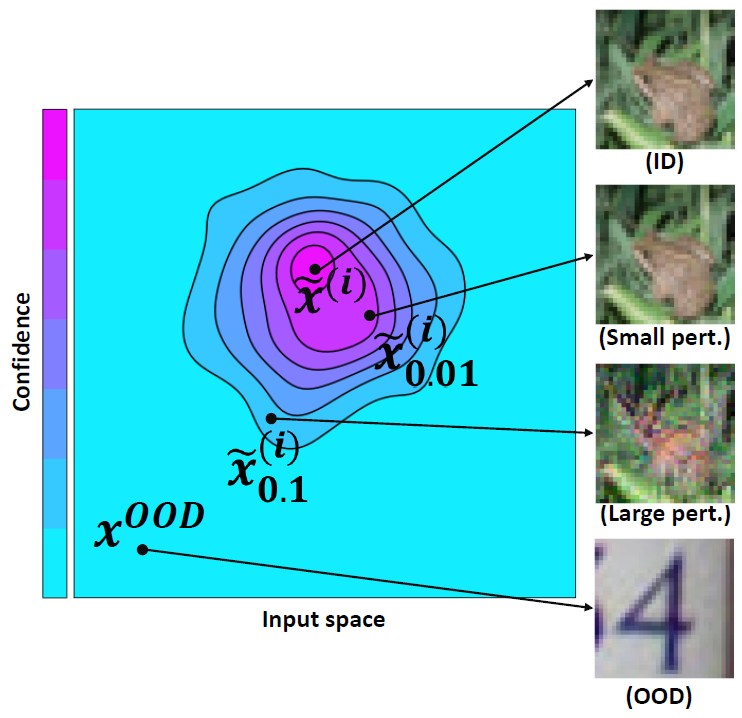
\includegraphics[width=0.36\textwidth]{sections/008_icml2021/eval/uncertainty_diagram.png}
\caption{Visualization of the desired uncertainty estimates. 
}
\label{fig:uncertainty_attack_diagram}
\end{figure}
%
DBU models have the advantage that they provide both, aleatoric uncertainty estimates resulting from irreducible uncertainty (e.g. class overlap or noise) and epistemic uncertainty estimates resulting from the lack of knowledge about unseen data (e.g. an unknown object is presented to the model). Both uncertainty types can be quantified from Dirichlet distributions using different uncertainty measures such as differential entropy, mutual information, or pseudo-counts. These uncertainty measures show outstanding performance in, e.g., the detection of OOD samples and thus are superior to softmax based confidence \citep{malini2018, malinin2019, charpentier2020}.

Neural networks from the families outlined above are expected to \emph{know what they don't know}, i.e. they are supposed to notice when they are unsure about a prediction. 
This raises questions with regards to adversarial examples: should uncertainty estimation methods \emph{detect} these corrupted samples by indicating a high uncertainty on them and abstain from making a prediction? Or should uncertainty estimation be \emph{robust} to adversarial examples and assign the correct label even under perturbations? We argue that being robust to adversarial perturbations is the best option (see Figure~\ref{fig:uncertainty_attack_diagram}) for two reasons. First, in image classification a human is usually not able to observe any difference between an adversarial example and an unperturbed image. Second, the size of the perturbation corresponding to a good adversarial example is typically small w.r.t.\ the $L_p$-norm and thus assumed to be semantically meaningless. 
Importantly, robustness should not only be required for the class predictions, but also for the uncertainty estimates. This means that DBU models should be able to distinguish robustly between ID and OOD data even if those are perturbed. 
%Importantly, one should require robustness not only for the class predictions, but also for the uncertainty estimation. This means that DBU models should be able to distinguish robustly between ID and OOD data even if those are perturbed. 

In this work, we focus on DBU models and analyze their robustness capacity w.r.t. class predictions as well as uncertainty predictions. In doing so, we go beyond simple softmax output confidence by investigating advanced uncertainty measures such as differential entropy.
Specifically, we study the following questions: 
%
\begin{enumerate}
    \item \emph{Is low uncertainty a reliable indicator of correct predictions?}
    \item \emph{Can we use uncertainty estimates to detect label attacks on the class prediction?}
    \item \emph{Are uncertainty estimates such as differential entropy a robust feature for OOD detection?}
\end{enumerate}

In addressing these questions we place particular focus on adversarial perturbations of the input to evaluate the \emph{worst case} performance of the models on increasing complex data sets and attacks.
%
We evaluate robustness of DBU models w.r.t. to these three questions by comparing their performance on unperturbed and perturbed inputs. Perturbed inputs are obtained by computing \emph{label attacks} and \emph{uncertainty attacks}, which are a new type of attacks we propose.  While label attacks aim at changing the class prediction, uncertainty attacks aim at changing the uncertainty estimate such that ID data is marked as OOD data and vice versa.
%
In total, we performed more than $138,800$ attack settings to explore the robustness landscape of DBU models. Those settings cover different data sets, attack types, attack losses, attack radii, DBU model types and initialisation seeds.
%
Finally, we propose and evaluate median smoothing and adversarial training based on label attacks and uncertainty attacks to make DBU models more robust. Our median smoothing approach provides certificates on epistemic uncertainty measures such as differential entropy and allows to certify uncertainty estimation.  The code and further supplementary material is available online (\url{www.daml.in.tum.de/dbu-robustness}).




